\documentclass[11pt,a4paper]{article}

\usepackage[margin=2.5cm]{geometry}
\usepackage[T1]{fontenc}
\usepackage{lmodern}
\usepackage{amsmath,amssymb,booktabs,graphicx,hyperref}

\hypersetup{
    colorlinks=true,
    urlcolor=blue,
    linkcolor=black
}

\title{
When Does Adaptive Coordinate Sampling Pay for Itself?\\
\large Ridge-Regression Baselines and a Published ASCD Comparison
}
\author{Clara Ng}
\date{26 September 2026}

\begin{document}

\maketitle

\begin{abstract}
We study coordinate-selection rules for ridge regression under feature
scaling and correlation. A baseline experiment compares uniform sampling,
fixed Lipschitz sampling, periodically refreshed gradient-gain sampling,
and a progress-triggered gradient-gain heuristic across four synthetic
regimes and the packaged diabetes regression dataset. Each method is
evaluated over 12 seeded runs using a common coordinate update and a
2,400-update budget. The two gradient-gain heuristics succeed on the
independent synthetic designs but fail to reach the target on either
correlated synthetic design within this budget.

As a subsequent published-method comparison, we implement the selection
mechanism of Approximate Steepest Coordinate Descent (ASCD) of Stich,
Raj, and Jaggi using their zero oracle with exact full-gradient
initialization, while retaining the benchmark's ridge coordinate update.
ASCD reaches the target in all 12 runs on three of the four synthetic
cases and on the diabetes dataset, and in 9 of 12 runs on the
scaled-correlated case, compared with 6 of 12 for uniform sampling
there. On the five scaled-correlated seeds where both methods reach the
target, ASCD records greater proxy work on every seed under the current
accounting convention. Its median active set also remains the full 48
coordinates on all four synthetic cases. The experiment therefore does
not establish a general computational advantage for adaptive selection.
It is a comparison on our benchmark rather than a reproduction of the
published ASCD experiments, and no claim of algorithmic novelty or
general superiority is made.
\end{abstract}


\section{Motivation and related work}

Randomized updates and adaptive information collection feature in
stochastic block BFGS \cite{gower2016}, minibatch semi-stochastic
optimization \cite{konecny2016}, parallel and accelerated coordinate
descent \cite{richtarik2016,fercoq2015}, and randomized linear solvers
\cite{gower2015}. Adaptive coordinate-selection methods include adaptive
probabilities for stochastic dual coordinate ascent \cite{csiba2015},
adaptive importance sampling \cite{perekrestenko2017}, and Approximate
Steepest Coordinate Descent (ASCD) \cite{stich2017}. These works prevent
gradient-informed sampling or refreshes alone from being treated as a
new idea.

The practical question in the baseline experiment is whether the benefit
of refreshing a sampling rule compensates for its additional computation
under feature scaling and correlation. After completing that baseline,
we additionally implement one published ASCD configuration and compare
it under the same frozen benchmark. This second experiment is a
cross-method comparison under our settings, not a reproduction of the
published ASCD figures.


\section{Experimental setup and baseline methods}

For a design matrix $X\in\mathbb{R}^{n\times d}$ and response $y$, we
minimize
\begin{equation}
f(w)=
\frac{1}{2}\lVert Xw-y\rVert_2^2+
\frac{\lambda}{2}\lVert w\rVert_2^2,
\qquad
\lambda=0.03.
\end{equation}

With residual $r=Xw-y$,
\begin{equation}
g_j=X_j^{\mathsf T}r+\lambda w_j,
\qquad
L_j=\lVert X_j\rVert_2^2+\lambda,
\end{equation}
and each baseline method applies
\begin{equation}
w_j \leftarrow w_j-\frac{g_j}{L_j}
\end{equation}
and updates the residual.

Uniform sampling uses $p_j=1/d$, whereas fixed Lipschitz sampling uses
\[
p_j=\frac{L_j}{\sum_k L_k}.
\]
Both gradient-gain variants use
\begin{equation}
p_j=
\frac{0.05}{d}
+
0.95
\frac{g_j^2/L_j}{\sum_k g_k^2/L_k},
\end{equation}
with uniform fallback when the denominator vanishes.

Scheduled gain refreshes initially and every 60 updates. Triggered gain
refreshes at step zero and subsequently at a 120-step checkpoint if the
latest objective decrease is below half the preceding decrease, subject
to a 60-step minimum interval. The trigger observes the objective rather
than the reference optimum.

The four synthetic cases cross balanced versus geometrically scaled
features with independent versus eight-group correlated features, with
$n=400$ and $d=48$. The packaged diabetes design provides a fifth case.
Each method uses 12 problem seeds and at most 2,400 coordinate updates.

A dense ridge solve defines $f^\ast$ for evaluation. A run succeeds if
a saved checkpoint satisfies
\[
f(w)-f^\ast \leq 10^{-4}.
\]
The reference optimum is used only for evaluation and not by the
selection rules.

For the baseline methods, the workload proxy counts $2n+3$ units per
coordinate update, $d$ per coordinate draw, $nd+d$ per probability
refresh, and $n+d$ per objective checkpoint. These units are bookkeeping
quantities rather than measured floating-point-operation counts.


\section{Baseline results}

\begin{table}[ht]
\centering
\caption{Baseline runs reaching the target within the 2,400-update
budget (out of 12).}
\label{tab:baseline-success}
\begin{tabular}{lrrrr}
\toprule
Case & Uniform & Lipschitz & Scheduled & Triggered \\
\midrule
Balanced independent & 12 & 12 & 12 & 12 \\
Scaled independent   & 12 &  0 & 12 & 12 \\
Balanced correlated  & 12 & 12 &  0 &  0 \\
Scaled correlated    &  6 &  0 &  0 &  0 \\
Diabetes             & 12 & 12 &  9 &  5 \\
\bottomrule
\end{tabular}
\end{table}

Uniform and fixed Lipschitz sampling both succeed in all runs of the
balanced-independent, balanced-correlated, and diabetes cases.
Lipschitz sampling fails on the scaled-independent case, where the other
three baseline methods succeed. The two gradient-gain heuristics fail
to reach the target in either correlated synthetic case within the
update budget.

Median time and work to target in the baseline summary use successful
runs only. Consequently, such conditional summaries must be interpreted
together with the corresponding success counts.

\begin{figure}[ht]
\centering
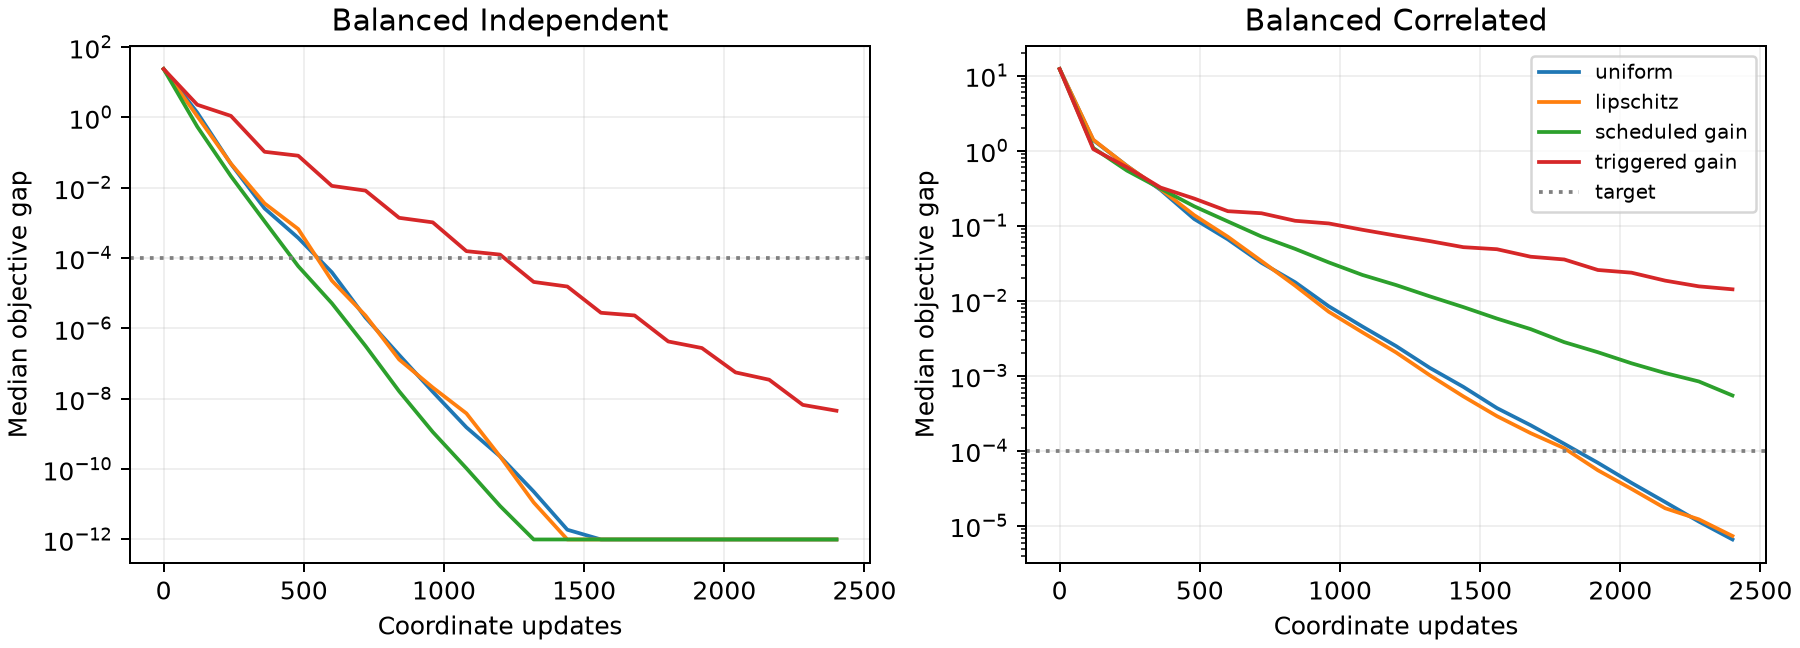
\includegraphics[width=\linewidth]{../results/median_trajectories.png}
\caption{Median objective gaps for the two balanced baseline cases.
The horizontal dotted line marks the $10^{-4}$ target. A median
trajectory does not display the variability across individual runs.}
\label{fig:baseline-trajectories}
\end{figure}


\section{Published ASCD comparison}

\subsection{Selection rule}

We next implement a configuration of Approximate Steepest Coordinate
Descent (ASCD) \cite{stich2017}. For every coordinate $j$, ASCD maintains
an estimated gradient $\widetilde g_j$ and a certified radius $r_j$
satisfying
\[
|g_j-\widetilde g_j|\leq r_j.
\]
This gives the upper and lower bounds
\begin{equation}
u_j=|\widetilde g_j|+r_j,
\qquad
\ell_j=\max\{0,|\widetilde g_j|-r_j\}.
\end{equation}

The active set is the smallest nonempty subset $I$ for which every
excluded coordinate satisfies
\begin{equation}
u_j^2
<
\frac{1}{|I|}
\sum_{i\in I}\ell_i^2.
\end{equation}
Equality therefore does not permit exclusion. A coordinate is selected
uniformly from the members of $I$ attaining the largest lower bound.

Our implementation initializes $\widetilde g$ using the exact full
gradient and sets all radii to zero. This is an allowed ASCD
configuration discussed by Stich et al.; it differs from the default
zero-estimate, infinite-radius initialization in their Algorithm~1.


\subsection{Zero oracle and radius update}

For this experiment we use the paper's zero oracle for cross-coordinate
gradient changes. If coordinate $i$ changes by $h$, then for $j\neq i$
the ridge gradient changes by
\begin{equation}
g_j^{\mathrm{new}}-g_j
=
hX_j^{\mathsf T}X_i.
\end{equation}
Cauchy--Schwarz gives
\begin{equation}
|g_j^{\mathrm{new}}-g_j|
\leq
|h|\,\lVert X_j\rVert_2\,\lVert X_i\rVert_2.
\end{equation}
The implementation therefore leaves the corresponding estimated
cross-gradient unchanged and increases its certified radius by this
upper bound.

For the selected coordinate,
\[
h=-\frac{g_i}{L_i},
\]
so exact minimization along that coordinate gives
\[
g_i^{\mathrm{new}}
=
g_i+hL_i
=
0
\]
up to numerical precision. Its estimate and radius can therefore be
reset to zero.


\subsection{Implementation verification}

The implementation includes a small-problem numerical audit. After
every audited update, it recomputes
\[
X^{\mathsf T}(Xw-y)+\lambda w
\]
and verifies that each true coordinate gradient lies inside its
maintained interval. It also verifies the residual invariant
$r=Xw-y$.

A manual active-set trace gives the same result as the implementation.
For example, with exact estimates
\[
\widetilde g=(3,1,0),\qquad r=(0,0,0),
\]
the initial mean squared lower bound is $10/3$. The zero coordinate can
therefore be excluded. For the remaining two coordinates the mean is
$5$, so the coordinate with squared upper bound $1$ can also be
excluded, leaving only the coordinate with gradient magnitude $3$.

Two useful additional automated audit checks are an explicit
equality-boundary test for the strict exclusion condition and an
assertion that the objective is nonincreasing after each audited exact
coordinate minimization.


\subsection{ASCD results}

The ASCD comparison uses the same five cases, 12 problem seeds,
initial point, objective, $10^{-4}$ target, 120-update checkpoint
spacing, and 2,400-update limit as the baseline.

\begin{table}[ht]
\centering
\caption{Uniform and ASCD results on the frozen benchmark. Work to
target is the median among successful runs under each method's recorded
proxy.}
\label{tab:ascd-results}
\begin{tabular}{lrrrrr}
\toprule
Case &
\multicolumn{2}{c}{Uniform} &
\multicolumn{3}{c}{ASCD} \\
\cmidrule(lr){2-3}\cmidrule(lr){4-6}
&
Success &
Work &
Success &
Work &
Median $|I|$ \\
\midrule
Balanced independent & 12/12 & 513,288   & 12/12 & 762,936   & 48 \\
Scaled independent   & 12/12 & 513,288   & 12/12 & 762,936   & 48 \\
Balanced correlated  & 12/12 & 1,641,536 & 12/12 & 2,249,416 & 48 \\
Scaled correlated    &  6/12 & 1,897,956 &  9/12 & 2,844,008 & 48 \\
Diabetes             & 12/12 & 919,234   & 12/12 & 984,864   & 10 \\
\bottomrule
\end{tabular}
\end{table}

ASCD reaches the target in all 12 runs on the balanced-independent,
scaled-independent, balanced-correlated, and diabetes cases. On the
scaled-correlated case it reaches the target in 9 of 12 runs, compared
with 6 of 12 for uniform sampling.

The work-to-target medians in Table~\ref{tab:ascd-results} are
conditional on successful runs. In particular, the scaled-correlated
uniform and ASCD medians are calculated from different sets of
successful problem seeds, so those two aggregate values alone are not
a paired cost comparison.

The active-set measurements are also informative. The median active
set is 48, the full coordinate dimension, on all four synthetic cases.
It is 10 on the 10-feature diabetes case. Thus this zero-oracle
configuration shows little active-set pruning under the synthetic
settings. The relatively broad certified Cauchy--Schwarz bounds are a
plausible mechanism, but a direct per-step analysis would be required
to establish the cause.


\subsection{Paired scaled-correlated comparison}

Because the uniform and ASCD successful-run medians in
Table~\ref{tab:ascd-results} are calculated from different subsets of
problem seeds, we additionally compare the methods seed by seed on the
scaled-correlated case. For each method and seed, work to target is the
proxy work recorded at the first saved checkpoint satisfying
$f(w)-f^\ast\leq 10^{-4}$.

Among the 12 paired problem seeds, uniform reaches the target on
6 seeds, whereas ASCD reaches it on 9. The two methods both reach the
target on five seeds: 0, 4, 5, 6, and 10. On these shared successes,
the median recorded work to target is 1,846,672 for uniform and
2,844,008 for ASCD. The median paired ASCD-minus-uniform difference is
997,336 proxy units, corresponding to a median ASCD/uniform recorded-work
ratio of 1.5401. ASCD records greater proxy work on all five shared
successes.

The paired runs also distinguish success-set differences. Seed 3 reaches
the target under uniform sampling but not under ASCD, whereas seeds 1,
7, 8, and 9 reach the target under ASCD but not under uniform sampling.
Thus the higher ASCD success count is not obtained simply by reproducing
the same successful instances.

This paired result separates two observations. Under the fixed
2,400-update budget, ASCD succeeds on more scaled-correlated problem
instances. On instances where both methods succeed, however, the
current proxy accounting does not show a lower work-to-target cost for
ASCD. The median recorded ASCD work on the shared successes is about
1.54 times the corresponding uniform median under the current accounting
conventions. These are descriptive results under the present cost model;
because setup and accounting boundaries are not fully harmonized, they
should not be interpreted as exact operation-count or wall-clock
superiority claims.


\subsection{Work accounting}

ASCD includes an initial full-gradient charge of
\[
nd+d
\]
proxy units. Each saved objective checkpoint adds $n+d$. Each coordinate
update adds
\[
2n+3+d\lceil\log_2 d\rceil+3d,
\]
representing the coordinate update, modelled sorting, and
bounds/interval maintenance.

These quantities are deliberately approximate bookkeeping units. Some
common matrix construction and data-generation work occurs outside the
timed ASCD method section, while ASCD's full-gradient initialization is
inside it. The baseline and ASCD timing/setup boundaries are therefore
not sufficiently harmonized to support a controlled wall-clock or exact
operation-count superiority claim.

The paired comparison above therefore uses the proxies exactly as
recorded by the two implementations, but it does not remove the
difference in accounting conventions. The resulting work differences
are descriptive under this cost model rather than controlled FLOP or
wall-clock comparisons.


\section{Interpretation and limitations}

The baseline results show that neither gradient-gain heuristic has a
consistent advantage over the fixed rules. In particular, both fail to
reach the target in the correlated synthetic regimes within the
2,400-update budget.

The published ASCD comparison changes the picture but does not establish
a general computational advantage. ASCD reaches the target in more
scaled-correlated runs than uniform sampling under the fixed update
budget. The paired analysis shows that, on the five scaled-correlated
instances where both methods succeed, ASCD records greater proxy work
on every instance under the present accounting convention. Moreover,
the median active set remains the entire coordinate set on all synthetic
cases. Under this zero-oracle configuration, the additional machinery
therefore does not translate into substantial observed pruning on these
problems.

The comparison has several limitations. Only one small packaged real
dataset is included, and no predictive generalization performance is
evaluated. The baseline trigger threshold, refresh interval, and
probability floor are illustrative choices. Proxy work is an accounting
measure rather than an exact FLOP count, and wall-clock measurements
depend on both implementation and hardware. Objective gaps reported as
zero can reflect floating-point precision.

The ASCD experiment should also not be described as a reproduction of
the figures in Stich et al. Their ridge-regression experiments use
different synthetic settings and oracle configurations. A strict
reproduction would require the corresponding data generation,
initialization, oracle precision, step-size/update convention, and
plotting protocol.

Finally, the paper's theoretical one-step comparison assumes a shared
coordinate smoothness bound and a common update method across the
algorithms being compared. The present benchmark uses coordinate-specific
$L_j$ values and its existing exact coordinate-minimization update.
The paper's dominance result therefore should not be interpreted as a
theoretical guarantee for the experimental comparison reported here.


\section{Conclusion and future research}

The baseline study and an initial published-method comparison are now
complete. The baseline gradient-gain heuristics do not succeed
consistently across the five cases, with the correlated synthetic
regimes providing a useful failure case. The subsequent ASCD
implementation reaches the scaled-correlated target in 9 of 12 runs
under the same update budget, compared with 6 of 12 for uniform
sampling.

The paired comparison sharpens this result. Five scaled-correlated seeds
succeed under both methods, and ASCD records greater proxy work on each
of those five. Median work to target on the shared successes is
1,846,672 for uniform and 2,844,008 for ASCD, a median recorded-work
ratio of 1.5401. Together with the full-size median active sets on the
synthetic cases, this means that the current zero-oracle ASCD
configuration does not demonstrate a cost advantage under the present
work model, despite its higher success count under the fixed
coordinate-update budget.

The next useful step is therefore not to claim superiority or novelty,
but to sharpen the remaining cost and mechanism analysis. The paired
per-seed scaled-correlated comparison is now complete; remaining work
includes harmonizing setup and cost accounting and examining the
distribution of active-set sizes over individual updates. A subsequent
predeclared experiment could evaluate a tighter \emph{published} ASCD
oracle, such as an approximate inner-product oracle, while explicitly
charging its information-acquisition cost. Broader datasets, held-out
experimental settings, and repeated wall-clock measurements would be
needed before drawing stronger conclusions.

Any later methodological modification should be separated clearly from
the published-method comparison and evaluated under a predeclared
question and evaluation protocol. The internship research topic would
be determined with the faculty member if an application succeeds.


\paragraph{Acknowledgement and research provenance.}
AI assistance was used in developing the initial benchmark, the ASCD
implementation and audit, the paired-analysis workflow, and report text.
The code and generated output files accompany the report for
reproducibility. The ASCD active-set condition and gradient-radius
derivation were manually reviewed during Stage~3; descriptions of
independent authorship should reflect the author's actual personal
verification, decisions, and revisions. Applicable citation and
AI-disclosure requirements should be followed.


\begin{thebibliography}{9}

\bibitem{gower2016}
R. M. Gower, D. Goldfarb, and P. Richt\'arik.
Stochastic block BFGS: Squeezing more curvature out of data.
\emph{Proceedings of ICML}, 2016.
\url{https://proceedings.mlr.press/v48/gower16.pdf}.

\bibitem{konecny2016}
J. Kone\v{c}n\'y, J. Liu, P. Richt\'arik, and M. Tak\'a\v{c}.
Mini-batch semi-stochastic gradient descent in the proximal setting.
\emph{IEEE Journal of Selected Topics in Signal Processing}, 2016.
\url{https://www.pure.ed.ac.uk/ws/portalfiles/portal/26531306/07347336.pdf}.

\bibitem{richtarik2016}
P. Richt\'arik and M. Tak\'a\v{c}.
Parallel coordinate descent methods for big data optimization.
\emph{Mathematical Programming}, 2016.
\url{https://arxiv.org/abs/1212.0873}.

\bibitem{gower2015}
R. M. Gower and P. Richt\'arik.
Randomized iterative methods for linear systems.
\emph{SIAM Journal on Matrix Analysis and Applications}, 2015.
\url{https://arxiv.org/abs/1506.03296}.

\bibitem{fercoq2015}
O. Fercoq and P. Richt\'arik.
Accelerated, parallel, and proximal coordinate descent.
\emph{SIAM Journal on Optimization}, 2015.
\url{https://arxiv.org/abs/1312.5799}.

\bibitem{csiba2015}
D. Csiba, Z. Qu, and P. Richt\'arik.
Stochastic dual coordinate ascent with adaptive probabilities.
\url{https://arxiv.org/abs/1502.08053}.

\bibitem{perekrestenko2017}
D. Perekrestenko, V. Cevher, and M. Jaggi.
Faster coordinate descent via adaptive importance sampling.
\emph{Proceedings of AISTATS}, 2017.
\url{https://proceedings.mlr.press/v54/perekrestenko17a.html}.

\bibitem{stich2017}
S. U. Stich, A. Raj, and M. Jaggi.
Approximate steepest coordinate descent.
\emph{Proceedings of ICML}, 2017.
\url{https://proceedings.mlr.press/v70/stich17a.html}.

\end{thebibliography}

\end{document}
